% Options for packages loaded elsewhere
\PassOptionsToPackage{unicode}{hyperref}
\PassOptionsToPackage{hyphens}{url}
\PassOptionsToPackage{dvipsnames,svgnames,x11names}{xcolor}
%
\documentclass[
  letterpaper,
  DIV=11]{scrartcl}

\usepackage{amsmath,amssymb}
\usepackage{iftex}
\ifPDFTeX
  \usepackage[T1]{fontenc}
  \usepackage[utf8]{inputenc}
  \usepackage{textcomp} % provide euro and other symbols
\else % if luatex or xetex
  \usepackage{unicode-math}
  \defaultfontfeatures{Scale=MatchLowercase}
  \defaultfontfeatures[\rmfamily]{Ligatures=TeX,Scale=1}
\fi
\usepackage{lmodern}
\ifPDFTeX\else  
    % xetex/luatex font selection
\fi
% Use upquote if available, for straight quotes in verbatim environments
\IfFileExists{upquote.sty}{\usepackage{upquote}}{}
\IfFileExists{microtype.sty}{% use microtype if available
  \usepackage[]{microtype}
  \UseMicrotypeSet[protrusion]{basicmath} % disable protrusion for tt fonts
}{}
\makeatletter
\@ifundefined{KOMAClassName}{% if non-KOMA class
  \IfFileExists{parskip.sty}{%
    \usepackage{parskip}
  }{% else
    \setlength{\parindent}{0pt}
    \setlength{\parskip}{6pt plus 2pt minus 1pt}}
}{% if KOMA class
  \KOMAoptions{parskip=half}}
\makeatother
\usepackage{xcolor}
\setlength{\emergencystretch}{3em} % prevent overfull lines
\setcounter{secnumdepth}{5}
% Make \paragraph and \subparagraph free-standing
\ifx\paragraph\undefined\else
  \let\oldparagraph\paragraph
  \renewcommand{\paragraph}[1]{\oldparagraph{#1}\mbox{}}
\fi
\ifx\subparagraph\undefined\else
  \let\oldsubparagraph\subparagraph
  \renewcommand{\subparagraph}[1]{\oldsubparagraph{#1}\mbox{}}
\fi

\usepackage{color}
\usepackage{fancyvrb}
\newcommand{\VerbBar}{|}
\newcommand{\VERB}{\Verb[commandchars=\\\{\}]}
\DefineVerbatimEnvironment{Highlighting}{Verbatim}{commandchars=\\\{\}}
% Add ',fontsize=\small' for more characters per line
\usepackage{framed}
\definecolor{shadecolor}{RGB}{241,243,245}
\newenvironment{Shaded}{\begin{snugshade}}{\end{snugshade}}
\newcommand{\AlertTok}[1]{\textcolor[rgb]{0.68,0.00,0.00}{#1}}
\newcommand{\AnnotationTok}[1]{\textcolor[rgb]{0.37,0.37,0.37}{#1}}
\newcommand{\AttributeTok}[1]{\textcolor[rgb]{0.40,0.45,0.13}{#1}}
\newcommand{\BaseNTok}[1]{\textcolor[rgb]{0.68,0.00,0.00}{#1}}
\newcommand{\BuiltInTok}[1]{\textcolor[rgb]{0.00,0.23,0.31}{#1}}
\newcommand{\CharTok}[1]{\textcolor[rgb]{0.13,0.47,0.30}{#1}}
\newcommand{\CommentTok}[1]{\textcolor[rgb]{0.37,0.37,0.37}{#1}}
\newcommand{\CommentVarTok}[1]{\textcolor[rgb]{0.37,0.37,0.37}{\textit{#1}}}
\newcommand{\ConstantTok}[1]{\textcolor[rgb]{0.56,0.35,0.01}{#1}}
\newcommand{\ControlFlowTok}[1]{\textcolor[rgb]{0.00,0.23,0.31}{#1}}
\newcommand{\DataTypeTok}[1]{\textcolor[rgb]{0.68,0.00,0.00}{#1}}
\newcommand{\DecValTok}[1]{\textcolor[rgb]{0.68,0.00,0.00}{#1}}
\newcommand{\DocumentationTok}[1]{\textcolor[rgb]{0.37,0.37,0.37}{\textit{#1}}}
\newcommand{\ErrorTok}[1]{\textcolor[rgb]{0.68,0.00,0.00}{#1}}
\newcommand{\ExtensionTok}[1]{\textcolor[rgb]{0.00,0.23,0.31}{#1}}
\newcommand{\FloatTok}[1]{\textcolor[rgb]{0.68,0.00,0.00}{#1}}
\newcommand{\FunctionTok}[1]{\textcolor[rgb]{0.28,0.35,0.67}{#1}}
\newcommand{\ImportTok}[1]{\textcolor[rgb]{0.00,0.46,0.62}{#1}}
\newcommand{\InformationTok}[1]{\textcolor[rgb]{0.37,0.37,0.37}{#1}}
\newcommand{\KeywordTok}[1]{\textcolor[rgb]{0.00,0.23,0.31}{#1}}
\newcommand{\NormalTok}[1]{\textcolor[rgb]{0.00,0.23,0.31}{#1}}
\newcommand{\OperatorTok}[1]{\textcolor[rgb]{0.37,0.37,0.37}{#1}}
\newcommand{\OtherTok}[1]{\textcolor[rgb]{0.00,0.23,0.31}{#1}}
\newcommand{\PreprocessorTok}[1]{\textcolor[rgb]{0.68,0.00,0.00}{#1}}
\newcommand{\RegionMarkerTok}[1]{\textcolor[rgb]{0.00,0.23,0.31}{#1}}
\newcommand{\SpecialCharTok}[1]{\textcolor[rgb]{0.37,0.37,0.37}{#1}}
\newcommand{\SpecialStringTok}[1]{\textcolor[rgb]{0.13,0.47,0.30}{#1}}
\newcommand{\StringTok}[1]{\textcolor[rgb]{0.13,0.47,0.30}{#1}}
\newcommand{\VariableTok}[1]{\textcolor[rgb]{0.07,0.07,0.07}{#1}}
\newcommand{\VerbatimStringTok}[1]{\textcolor[rgb]{0.13,0.47,0.30}{#1}}
\newcommand{\WarningTok}[1]{\textcolor[rgb]{0.37,0.37,0.37}{\textit{#1}}}

\providecommand{\tightlist}{%
  \setlength{\itemsep}{0pt}\setlength{\parskip}{0pt}}\usepackage{longtable,booktabs,array}
\usepackage{calc} % for calculating minipage widths
% Correct order of tables after \paragraph or \subparagraph
\usepackage{etoolbox}
\makeatletter
\patchcmd\longtable{\par}{\if@noskipsec\mbox{}\fi\par}{}{}
\makeatother
% Allow footnotes in longtable head/foot
\IfFileExists{footnotehyper.sty}{\usepackage{footnotehyper}}{\usepackage{footnote}}
\makesavenoteenv{longtable}
\usepackage{graphicx}
\makeatletter
\def\maxwidth{\ifdim\Gin@nat@width>\linewidth\linewidth\else\Gin@nat@width\fi}
\def\maxheight{\ifdim\Gin@nat@height>\textheight\textheight\else\Gin@nat@height\fi}
\makeatother
% Scale images if necessary, so that they will not overflow the page
% margins by default, and it is still possible to overwrite the defaults
% using explicit options in \includegraphics[width, height, ...]{}
\setkeys{Gin}{width=\maxwidth,height=\maxheight,keepaspectratio}
% Set default figure placement to htbp
\makeatletter
\def\fps@figure{htbp}
\makeatother
% definitions for citeproc citations
\NewDocumentCommand\citeproctext{}{}
\NewDocumentCommand\citeproc{mm}{%
  \begingroup\def\citeproctext{#2}\cite{#1}\endgroup}
\makeatletter
 % allow citations to break across lines
 \let\@cite@ofmt\@firstofone
 % avoid brackets around text for \cite:
 \def\@biblabel#1{}
 \def\@cite#1#2{{#1\if@tempswa , #2\fi}}
\makeatother
\newlength{\cslhangindent}
\setlength{\cslhangindent}{1.5em}
\newlength{\csllabelwidth}
\setlength{\csllabelwidth}{3em}
\newenvironment{CSLReferences}[2] % #1 hanging-indent, #2 entry-spacing
 {\begin{list}{}{%
  \setlength{\itemindent}{0pt}
  \setlength{\leftmargin}{0pt}
  \setlength{\parsep}{0pt}
  % turn on hanging indent if param 1 is 1
  \ifodd #1
   \setlength{\leftmargin}{\cslhangindent}
   \setlength{\itemindent}{-1\cslhangindent}
  \fi
  % set entry spacing
  \setlength{\itemsep}{#2\baselineskip}}}
 {\end{list}}
\usepackage{calc}
\newcommand{\CSLBlock}[1]{\hfill\break\parbox[t]{\linewidth}{\strut\ignorespaces#1\strut}}
\newcommand{\CSLLeftMargin}[1]{\parbox[t]{\csllabelwidth}{\strut#1\strut}}
\newcommand{\CSLRightInline}[1]{\parbox[t]{\linewidth - \csllabelwidth}{\strut#1\strut}}
\newcommand{\CSLIndent}[1]{\hspace{\cslhangindent}#1}

\KOMAoption{captions}{tableheading}
\makeatletter
\@ifpackageloaded{caption}{}{\usepackage{caption}}
\AtBeginDocument{%
\ifdefined\contentsname
  \renewcommand*\contentsname{Inhaltsverzeichnis}
\else
  \newcommand\contentsname{Inhaltsverzeichnis}
\fi
\ifdefined\listfigurename
  \renewcommand*\listfigurename{Abbildungsverzeichnis}
\else
  \newcommand\listfigurename{Abbildungsverzeichnis}
\fi
\ifdefined\listtablename
  \renewcommand*\listtablename{Tabellenverzeichnis}
\else
  \newcommand\listtablename{Tabellenverzeichnis}
\fi
\ifdefined\figurename
  \renewcommand*\figurename{Abbildung}
\else
  \newcommand\figurename{Abbildung}
\fi
\ifdefined\tablename
  \renewcommand*\tablename{Tabelle}
\else
  \newcommand\tablename{Tabelle}
\fi
}
\@ifpackageloaded{float}{}{\usepackage{float}}
\floatstyle{ruled}
\@ifundefined{c@chapter}{\newfloat{codelisting}{h}{lop}}{\newfloat{codelisting}{h}{lop}[chapter]}
\floatname{codelisting}{Listing}
\newcommand*\listoflistings{\listof{codelisting}{Listingverzeichnis}}
\makeatother
\makeatletter
\makeatother
\makeatletter
\@ifpackageloaded{caption}{}{\usepackage{caption}}
\@ifpackageloaded{subcaption}{}{\usepackage{subcaption}}
\makeatother
\ifLuaTeX
\usepackage[bidi=basic]{babel}
\else
\usepackage[bidi=default]{babel}
\fi
\babelprovide[main,import]{ngerman}
% get rid of language-specific shorthands (see #6817):
\let\LanguageShortHands\languageshorthands
\def\languageshorthands#1{}
\ifLuaTeX
  \usepackage{selnolig}  % disable illegal ligatures
\fi
\usepackage{bookmark}

\IfFileExists{xurl.sty}{\usepackage{xurl}}{} % add URL line breaks if available
\urlstyle{same} % disable monospaced font for URLs
\hypersetup{
  pdftitle={Ein datenwissenschaftlicher Blogbeitrag},
  pdfauthor={Malte Hagener; Andrea Rapp},
  pdflang={de},
  colorlinks=true,
  linkcolor={blue},
  filecolor={Maroon},
  citecolor={Blue},
  urlcolor={Blue},
  pdfcreator={LaTeX via pandoc}}

\title{Ein datenwissenschaftlicher Blogbeitrag}
\usepackage{etoolbox}
\makeatletter
\providecommand{\subtitle}[1]{% add subtitle to \maketitle
  \apptocmd{\@title}{\par {\large #1 \par}}{}{}
}
\makeatother
\subtitle{Eine Reise durch einige Möglichkeiten von Quarto}
\author{Malte Hagener \and Andrea Rapp}
\date{2024-02-17}

\begin{document}
\maketitle

\renewcommand*\contentsname{Inhaltsverzeichnis}
{
\hypersetup{linkcolor=}
\setcounter{tocdepth}{3}
\tableofcontents
}
\section{Unser Blogbeitrag}\label{unser-blogbeitrag}

Dies ist ein Typoblindtext. An ihm kann man sehen, ob alle Buchstaben da
sind und wie sie aussehen. Manchmal benutzt man Worte wie Hamburgefonts,
Rafgenduks oder Handgloves, um Schriften zu testen. Manchmal Sätze, die
alle Buchstaben des Alphabets enthalten - man nennt diese Sätze
»Pangrams«. Sehr bekannt ist dieser: The quick brown fox jumps over the
lazy old dog. Oft werden in Typoblindtexte auch fremdsprachige Satzteile
eingebaut (AVAIL® and Wefox™ are testing aussi la Kerning), um die
Wirkung in anderen Sprachen zu testen. In Lateinisch sieht zum Beispiel
fast jede Schrift gut aus. Quod erat demonstrandum. Seit 1975 fehlen in
den meisten Testtexten die Zahlen, weswegen nach TypoGb. 204 § ab dem
Jahr 2034 Zahlen in 86 der Texte zur Pflicht werden. Nichteinhaltung
wird mit bis zu 245 € oder 368 \$ bestraft. Genauso wichtig in sind
mittlerweile auch Âçcèñtë, die in neueren Schriften aber fast immer
enthalten sind. Ein wichtiges aber schwierig zu integrierendes Feld sind
OpenType-Funktionalitäten. Je nach Software und Voreinstellungen können
eingebaute Kapitälchen, Kerning oder Ligaturen (sehr pfiffig) nicht
richtig dargestellt werden. Dies ist ein Typoblindtext.(Karsdorp,
Kestemont und Riddell 2021) An ihm kann man sehen, ob alle Buchstaben da
sind und wie sie aussehen. Manchmal benutzt man Worte wie Hamburgefonts,
Rafgenduks oder Handgloves, um Schriften zu testen. Manchmal Sätze, die
alle Buchstaben des Alphabets enthalten - man nennt diese Sätze
»Pangrams«. Sehr bekannt ist dieser: The quick brown fox jumps over the
lazy old dog. Oft werden in Typoblindtexte auch fremdsprachige Satzteile
eingebaut (AVAIL® and Wefox™ are testing aussi la Kerning), um die
Wirkung in anderen Sprachen zu testen. In Lateinisch sieht zum Beispiel
fast jede Schrift gut aus. Quod erat demonstrandum. Seit 1975 fehlen in
den meisten Testtexten die Zahlen, weswegen nach TypoGb. 204 § ab dem
Jahr 2034 Zahlen in 86 der Texte zur Pflicht werden. Nichteinhaltung
wird mit bis zu 245 € oder 368 \$ bestraft. Genauso wichtig in sind
mittlerweile auch Âçcèñtë, die in neueren Schriften aber fast immer
enthalten sind. Ein wichtiges aber schwierig zu integrierendes Feld sind
OpenType-Funktionalitäten. Je nach Software und Voreinstellungen können
eingebaute Kapitälchen, Kerning oder Ligaturen (sehr pfiffig) nicht
richtig dargestellt werden.

Dies ist ein Typoblindtext. An ihm kann man sehen, ob alle Buchstaben da
sind und wie sie aussehen. Manchmal benutzt man Worte wie Hamburgefonts,
Rafgenduks oder Handgloves, um Schriften zu testen. Manchmal Sätze, die
alle Buchstaben des Alphabets enthalten - man nennt diese Sätze
»Pangrams«. Sehr bekannt ist dieser: The quick brown fox jumps over the
lazy old dog. Oft werden in Typoblindtexte auch fremdsprachige Satzteile
eingebaut (AVAIL® and Wefox™ are testing aussi la Kerning), um die
Wirkung in anderen Sprachen zu testen. In Lateinisch sieht zum Beispiel
fast jede Schrift gut aus. Quod erat demonstrandum. Seit 1975 fehlen in
den meisten Testtexten die Zahlen, weswegen nach TypoGb. 204 § ab dem
Jahr 2034 Zahlen in 86 der Texte zur Pflicht werden. Nichteinhaltung
wird mit bis zu 245 € oder 368 \$ bestraft. Genauso wichtig in sind
mittlerweile auch Âçcèñtë, die in neueren Schriften aber fast immer
enthalten sind. Ein wichtiges aber schwierig zu integrierendes Feld sind
OpenType-Funktionalitäten.(Altenhöner u.~a. 2020) Je nach Software und
Voreinstellungen können eingebaute Kapitälchen, Kerning oder Ligaturen
(sehr pfiffig) nicht richtig dargestellt werden.

\subsection{Überschrift 2}\label{uxfcberschrift-2}

Dies ist ein Typoblindtext. An ihm kann man sehen, ob alle Buchstaben da
sind und wie sie aussehen. Manchmal benutzt man Worte wie Hamburgefonts,
Rafgenduks oder Handgloves, um Schriften zu testen. Manchmal Sätze, die
alle Buchstaben des Alphabets enthalten - man nennt diese Sätze
»Pangrams«. Sehr bekannt ist dieser: The quick brown fox jumps over the
lazy old dog. Oft werden in Typoblindtexte auch fremdsprachige Satzteile
eingebaut (AVAIL® and Wefox™ are testing aussi la Kerning), um die
Wirkung in anderen Sprachen zu testen. In Lateinisch sieht zum Beispiel
fast jede Schrift gut aus. Quod erat demonstrandum. Seit 1975 fehlen in
den meisten Testtexten die Zahlen, weswegen nach TypoGb. 204 § ab dem
Jahr 2034 Zahlen in 86 der Texte zur Pflicht werden. Nichteinhaltung
wird mit bis zu 245 € oder 368 \$ bestraft. Genauso wichtig in sind
mittlerweile auch Âçcèñtë, die in neueren Schriften aber fast immer
enthalten sind. Ein wichtiges aber schwierig zu integrierendes Feld sind
OpenType-Funktionalitäten. Je nach Software und Voreinstellungen können
eingebaute Kapitälchen, Kerning oder Ligaturen (sehr pfiffig) nicht
richtig dargestellt werden.

Siehe Tabelle~\ref{tbl-panel} und für weitere Details insbesondere
Tabelle~\ref{tbl-second}.

Dies ist ein Typoblindtext. An ihm kann man sehen, ob alle Buchstaben da
sind und wie sie aussehen. Manchmal benutzt man Worte wie Hamburgefonts,
Rafgenduks oder Handgloves, um Schriften zu testen. Manchmal Sätze, die
alle Buchstaben des Alphabets enthalten - man nennt diese Sätze
»Pangrams«. Sehr bekannt ist dieser: The quick brown fox jumps over the
lazy old dog. Oft werden in Typoblindtexte(Zweig 2019) auch
fremdsprachige Satzteile eingebaut (AVAIL® and Wefox™ are testing aussi
la Kerning), um die Wirkung in anderen Sprachen zu testen. In Lateinisch
sieht zum Beispiel fast jede Schrift gut aus. Quod erat demonstrandum.
Seit 1975 fehlen in den meisten Testtexten die Zahlen, weswegen nach
TypoGb. 204 § ab dem Jahr 2034 Zahlen in 86 der Texte zur Pflicht
werden. Nichteinhaltung wird mit bis zu 245 € oder 368 \$ bestraft.
Genauso wichtig in sind mittlerweile auch Âçcèñtë, die in neueren
Schriften aber fast immer enthalten sind. Ein wichtiges aber schwierig
zu integrierendes Feld sind OpenType-Funktionalitäten. Je nach Software
und Voreinstellungen können eingebaute Kapitälchen, Kerning oder
Ligaturen (sehr pfiffig) nicht richtig dargestellt werden.

\begin{table}

\caption{\label{tbl-panel}Enorm wichtige Daten.}

\begin{minipage}{0.50\linewidth}

\subcaption{\label{tbl-first}Wichtige Daten}

\centering{

\begin{tabular}{lll}
\toprule
Col1 & Col2 & Col3\\
\midrule
A & B & C\\
E & F & G\\
A & G & G\\
\bottomrule
\end{tabular}

}

\end{minipage}%
%
\begin{minipage}{0.50\linewidth}

\subcaption{\label{tbl-second}Die entscheidenden Details}

\centering{

\begin{tabular}{lll}
\toprule
Col1 & Col2 & Col3\\
\midrule
A & B & C\\
E & F & G\\
A & G & G\\
\bottomrule
\end{tabular}

}

\end{minipage}%

\end{table}%

\section{Einbindung von Code und
Notebooks}\label{einbindung-von-code-und-notebooks}

Dies ist ein Typoblindtext. An ihm kann man sehen, ob alle Buchstaben da
sind und wie sie aussehen. Manchmal benutzt man Worte wie Hamburgefonts,
Rafgenduks oder Handgloves, um Schriften zu testen. Manchmal Sätze, die
alle Buchstaben des Alphabets enthalten - man nennt diese Sätze
»Pangrams«.(Manovich 2020) Sehr bekannt ist dieser: The quick brown fox
jumps over the lazy old dog. Oft werden in Typoblindtexte auch
fremdsprachige Satzteile eingebaut (AVAIL® and Wefox™ are testing aussi
la Kerning), um die Wirkung in anderen Sprachen zu testen. In Lateinisch
sieht zum Beispiel fast jede Schrift gut aus. Quod erat demonstrandum.
Seit 1975 fehlen in den meisten Testtexten die Zahlen, weswegen nach
TypoGb. 204 § ab dem Jahr 2034 Zahlen in 86 der Texte zur Pflicht
werden. Nichteinhaltung wird mit bis zu 245 € oder 368 \$ bestraft.
Genauso wichtig in sind mittlerweile auch Âçcèñtë, die in neueren
Schriften aber fast immer enthalten sind. Ein wichtiges aber schwierig
zu integrierendes Feld sind OpenType-Funktionalitäten. Je nach Software
und Voreinstellungen können eingebaute Kapitälchen, Kerning oder
Ligaturen (sehr pfiffig) nicht richtig dargestellt werden.

\subsection{Ein bisschen Python
gefällig?}\label{ein-bisschen-python-gefuxe4llig}

Wir können auch Python-Code mit Quarto darstellen (s.
Abbildung~\ref{fig-fibo})!

\begin{figure}

\centering{

\begin{Shaded}
\begin{Highlighting}[]
\KeywordTok{def}\NormalTok{ fib(n):}
    \ControlFlowTok{if}\NormalTok{ n }\OperatorTok{\textless{}} \DecValTok{1}\NormalTok{:}
        \ControlFlowTok{raise} \PreprocessorTok{Exception}\NormalTok{(}\StringTok{\textquotesingle{}undefined\textquotesingle{}}\NormalTok{)}
    \ControlFlowTok{elif}\NormalTok{ n }\OperatorTok{\textless{}} \DecValTok{3}\NormalTok{:}
        \ControlFlowTok{return} \DecValTok{1}
    \ControlFlowTok{else}\NormalTok{:}
        \ControlFlowTok{return}\NormalTok{ fib(n}\OperatorTok{{-}}\DecValTok{1}\NormalTok{) }\OperatorTok{+}\NormalTok{ fib(n}\OperatorTok{{-}}\DecValTok{2}\NormalTok{)}
\end{Highlighting}
\end{Shaded}

}

\caption{\label{fig-fibo}Rekursive Funktion zur Berechnung von
Fibonacci-Zahlen.}

\end{figure}%

Wir können aber auch Python-Code ausführen lassen und z.B. eine
Visualisierung mit matplotlib erzeugen, s. Abbildung~\ref{fig-polar}.

\begin{Shaded}
\begin{Highlighting}[]
\ImportTok{import}\NormalTok{ numpy }\ImportTok{as}\NormalTok{ np}
\ImportTok{import}\NormalTok{ matplotlib.pyplot }\ImportTok{as}\NormalTok{ plt}

\NormalTok{r }\OperatorTok{=}\NormalTok{ np.arange(}\DecValTok{0}\NormalTok{, }\DecValTok{2}\NormalTok{, }\FloatTok{0.01}\NormalTok{)}
\NormalTok{theta }\OperatorTok{=} \DecValTok{2} \OperatorTok{*}\NormalTok{ np.pi }\OperatorTok{*}\NormalTok{ r}
\NormalTok{fig, ax }\OperatorTok{=}\NormalTok{ plt.subplots(}
\NormalTok{  subplot\_kw }\OperatorTok{=}\NormalTok{ \{}\StringTok{\textquotesingle{}projection\textquotesingle{}}\NormalTok{: }\StringTok{\textquotesingle{}polar\textquotesingle{}}\NormalTok{\} }
\NormalTok{)}
\NormalTok{ax.plot(theta, r)}
\NormalTok{ax.set\_rticks([}\FloatTok{0.5}\NormalTok{, }\DecValTok{1}\NormalTok{, }\FloatTok{1.5}\NormalTok{, }\DecValTok{2}\NormalTok{])}
\NormalTok{ax.grid(}\VariableTok{True}\NormalTok{)}
\NormalTok{plt.show()}
\end{Highlighting}
\end{Shaded}

\begin{figure}[H]

\centering{

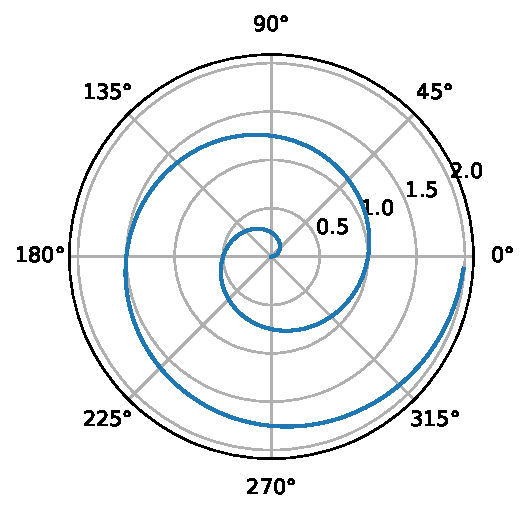
\includegraphics{index_files/figure-pdf/fig-polar-output-1.pdf}

}

\caption{\label{fig-polar}A line plot on a polar axis}

\end{figure}%

Dies ist ein Typoblindtext. An ihm kann man sehen, ob alle Buchstaben da
sind und wie sie aussehen. Manchmal benutzt man Worte wie Hamburgefonts,
Rafgenduks oder Handgloves, um Schriften zu testen. Manchmal Sätze, die
alle Buchstaben des Alphabets enthalten - man nennt diese Sätze
»Pangrams«. Sehr bekannt ist dieser: The quick brown fox jumps over the
lazy old dog. Oft werden in Typoblindtexte auch fremdsprachige Satzteile
eingebaut (AVAIL® and Wefox™ are testing aussi la Kerning), um die
Wirkung in anderen Sprachen zu testen. In Lateinisch sieht zum Beispiel
fast jede Schrift gut aus. Quod erat demonstrandum. Seit 1975 fehlen in
den meisten Testtexten die Zahlen, weswegen nach TypoGb. 204 § ab dem
Jahr 2034 Zahlen in 86 der Texte zur Pflicht werden. Nichteinhaltung
wird mit bis zu 245 € oder 368 \$ bestraft. Genauso wichtig in sind
mittlerweile auch Âçcèñtë(Cremer, Klaffki und Steyer 2018), die in
neueren Schriften aber fast immer enthalten sind. Ein wichtiges aber
schwierig zu integrierendes Feld sind OpenType-Funktionalitäten. Je nach
Software und Voreinstellungen können eingebaute Kapitälchen, Kerning
oder Ligaturen (sehr pfiffig) nicht richtig dargestellt werden. Dies ist
ein Typoblindtext. An ihm kann man sehen, ob alle Buchstaben da sind und
wie sie aussehen. Manchmal benutzt man Worte wie Hamburgefonts,
Rafgenduks oder Handgloves, um Schriften zu testen. Manchmal Sätze, die
alle Buchstaben des Alphabets enthalten - man nennt diese Sätze
»Pangrams«. Sehr bekannt ist dieser: The quick brown fox jumps over the
lazy old dog. Oft werden in Typoblindtexte auch fremdsprachige Satzteile
eingebaut (AVAIL® and Wefox™ are testing aussi la Kerning), um die
Wirkung in anderen Sprachen zu testen. In Lateinisch sieht zum Beispiel
fast jede Schrift gut aus. Quod erat demonstrandum. Seit 1975 fehlen in
den meisten Testtexten die Zahlen, weswegen nach TypoGb. 204 § ab dem
Jahr 2034 Zahlen in 86 der Texte zur Pflicht werden. Nichteinhaltung
wird mit bis zu 245 € oder 368 \$ bestraft. Genauso wichtig in sind
mittlerweile auch Âçcèñtë, die in neueren Schriften aber fast immer
enthalten sind. Ein wichtiges aber schwierig zu integrierendes Feld sind
OpenType-Funktionalitäten. Je nach Software und Voreinstellungen können
eingebaute Kapitälchen, Kerning oder Ligaturen (sehr pfiffig) nicht
richtig dargestellt werden.

Wir können auch Code aus einem Jupyter-Notebook einbinden:

\begin{figure}

\centering{

\begin{verbatim}
alt.Chart(...)
\end{verbatim}

}

\caption{\label{fig-bill-scatter}A scatterplot of bill dimensions for
penguins, made with Altair.}

\end{figure}%

\section{Eine weitere Überschrift}\label{eine-weitere-uxfcberschrift}

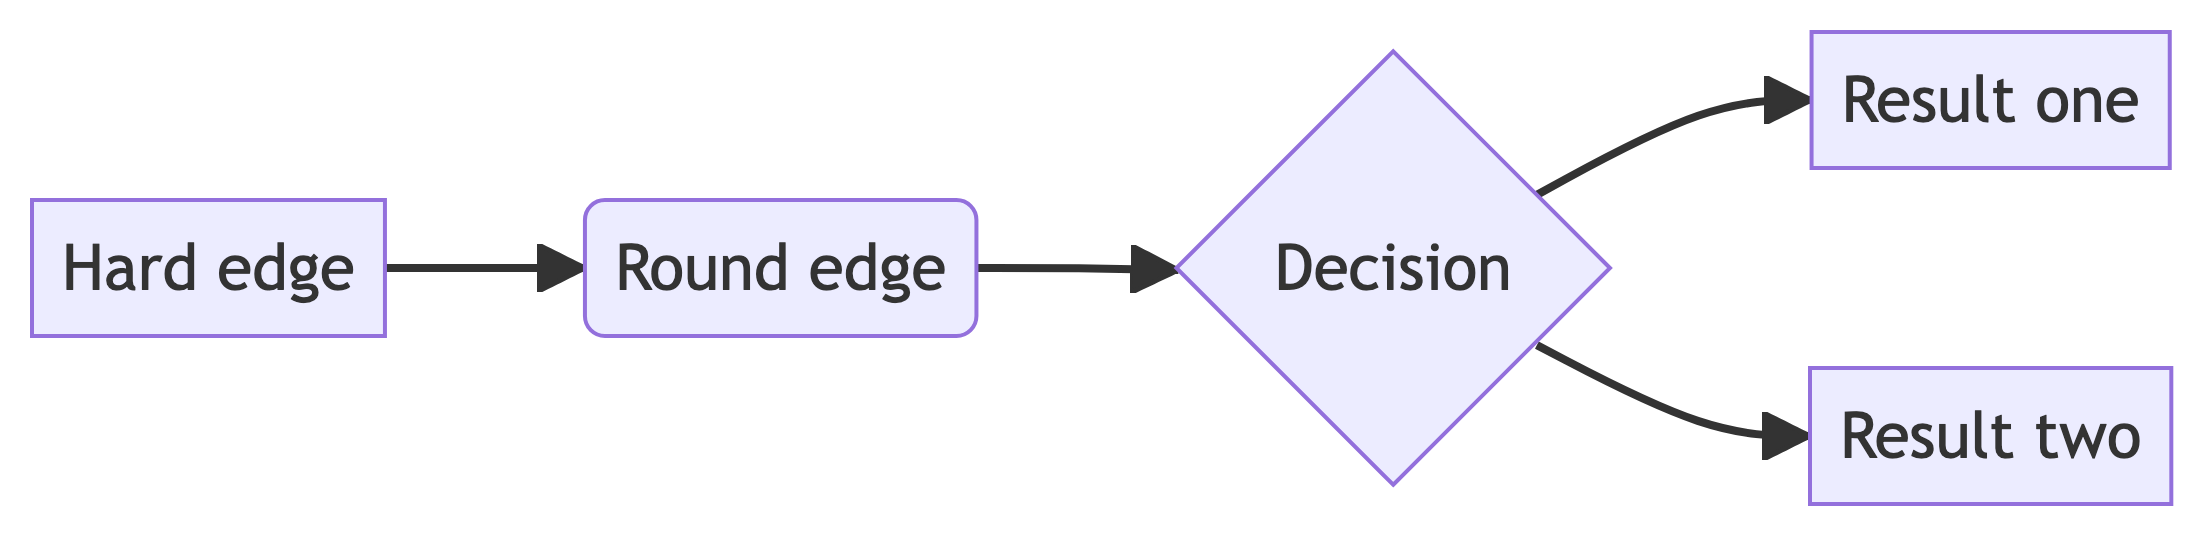
\includegraphics[width=5.74in,height=1.4in]{index_files/figure-latex/mermaid-figure-1.png}

Ein beispielhaftes Diagramm.

\section{Bibliographie}\label{bibliographie}

\phantomsection\label{refs}
\begin{CSLReferences}{1}{0}
\bibitem[\citeproctext]{ref-altenhoner_nfdi4culture_2020}
Altenhöner, Reinhard, Ina Blümel, Franziska Boehm, Jens Bove, Katrin
Bicher, Christian Bracht, Ortrun Brand, u.~a. 2020. {NFDI4Culture} -
{Consortium} for research data on material and immaterial cultural
heritage. \emph{Research Ideas and Outcomes} 6 (Juli): e57036.
doi:\href{https://doi.org/10.3897/rio.6.e57036}{10.3897/rio.6.e57036},
\url{https://riojournal.com/article/57036/} (zugegriffen: 20. Februar
2023).

\bibitem[\citeproctext]{ref-cremer_chimare_2018}
Cremer, Fabian, Lisa Klaffki und Timo Steyer. 2018. Der {Chimäre} auf
der {Spur}: {Forschungsdaten} in den {Geisteswissenschaften}.
\emph{o-bib. Das offene Bibliotheksjournal / Herausgeber VDB} (Juli):
142--162 Seiten.
doi:\href{https://doi.org/10.5282/O-BIB/2018H2S142-162}{10.5282/O-BIB/2018H2S142-162},
\url{https://www.o-bib.de/article/view/2018H2S142-162} (zugegriffen: 21.
Februar 2023).

\bibitem[\citeproctext]{ref-karsdorp_humanities_2021}
Karsdorp, Folgert, Mike Kestemont und Allen Riddell. 2021.
\emph{Humanities {Data} {Analysis}: {Case} {Studies} with {Python}}.
Princeton University Press.
\url{https://press.princeton.edu/books/hardcover/9780691172361/humanities-data-analysis}
(zugegriffen: 19. Mai 2021).

\bibitem[\citeproctext]{ref-manovich_cultural_2020}
Manovich, Lev. 2020. \emph{Cultural {Analytics}}. The MIT Press.

\bibitem[\citeproctext]{ref-zweig_algorithmus_2019}
Zweig, Katharina A. 2019. \emph{Ein {Algorithmus} hat kein {Taktgefühl}:
{Wo} künstliche {Intelligenz} sich irrt, warum uns das betrifft und was
wir dagegen tun können}. Heyne Verlag.

\end{CSLReferences}



\end{document}
